\chapter{Introduction}
	\label{chap:intro}
	For many years, IT professionals have preached the importance of strong passwords. Many publications exist, describing exactly what defines a strong password. The general consensus is that it needs \emph{at least} both upper- and lower-case letters, digits and preferably also symbols \emph{(\#, \_, etc.)}. Additionally, it shouldn't be a word -- or a word where an L is replaced by a 1. And of course it has to be at least 8 characters long. And you're not supposed to use the same password more than once place. With all of these rules for strong passwords, it is hardly a surprise that a lot of the regular users of IT systems resort to simple and repetitive passwords.

	To help alleviate this problem, a new class of software grew popular: Password managers. Simple tools, protected by a single master password, which generate and store passwords in a secure manner. A lot of the IT professionals took these tools to their heart, despite their inherent flaws. 

	As with so many other things in modern society, the users crave convenience. Tools storing an encrypted file locally, was no longer sufficient, as the majority of users began to use multiple devices. Hence, the password managers slowly migrated into The Cloud.

	\section{The Cloud}
		The origin of the term ``The Cloud'' stems from Cloud Computing. Computations too heavy to be performed on a single machine, were divided onto several -- usually networked -- machines, which then shared the computational load. However, when we say the cloud today, it is not \emph{exactly} this we think of.

		The concept of the cloud is simple: Your data, and any computations associated with it, is stored and performed somewhere \emph{else}: In the so called cloud.

		This saves the users from the hassle of managing this, themselves. Applications such as Dropbox, OneDrive and Google Drive is prime examples of what the cloud exactly is: You unload some of the ``responsibilities'' onto something, or someone else. Once that file has been dragged into your Dropbox folder, and that little icon is green instead of blue, you're safe. Your data is now kept for you, available at all times, from any device. It is in the cloud.

		While the cloud \emph{does} come with its benefits, especially convenience, it has its own drawbacks as well. Let us talk about \emph{trust}.

		\subsection*{Trust}
			When uploading data into the cloud, the user is effectively trusting the vendor. They're trusting that the vendor is completely honest regarding their inner workings, what they can access and what they can not access. They are trusting the vendor, when they say that they do not \emph{(or possibly do)} sell your information to a third party.

			Trusting vendors is completely fine. You can't access the web without a certain amount of trust. Just look at the worlds most popular search engine, Google. Unfortunately, sometimes this trust is betrayed.

			Dropbox experienced this, when users discovered that the data they uploaded to Dropbox, was in fact not so private. Using hashing techniques to discover duplicate files, they ``save'' the user's bandwidth, by using an already stored file on their server. While this does sound like a reasonable feature, it also means that Dropbox has access to the raw files on their server somehow, which again leads us to question the privacy of Dropbox.

			Another example of this misplaced trust, is the incident involving LastPass in 2015. As many IT professionals had feared, the online password manager had a breach. Panic arose and LastPass almost forced their users to change their passwords. Exactly this, is the general issue with the cloud. You have to trust someone else to store it.

			This is the general issue with the cloud: You trust someone else to store your confidential information. Someone else to ensure that your data does not end up in the hand of someone else.

	\section{The Private Cloud}
		To counteract these issues, more and more people started hosting \emph{(self-hosted)} applications themselves, giving them cloud-like features, without ever relinquishing control or ownership of their data. This concept has evolved, especially during the last few years, into something called the ``private cloud''. 

		While the private cloud originally was intended for the various corporations and enterprise solutions, more and more open-source solutions have started to emerge. These solutions target users, tired of having to practically sign over ownership of their data, to benefit from seamless multi-device integration. They aim to create functionality, previously limited to the public cloud, by \emph{only} using the user's own hardware.

		Unfortunately, running a private cloud come with its own set of issues. First and foremost there is the issue of finances: A server not only costs money to acquire, but also to run. To run a server 24/7, would cost a fair amount. Secondly, there's the issue of setting this private cloud up. 

		\subsection*{The Financial Cost of the Private Cloud}
			\label{sec:privatecloud_cost}
			Previously, it was only enthusiasts with their own private \emph{servers} who was able to host these applications. These servers could be made from anything between an old discarded PC, to top of the line server hardware which the enthusiasts chose to buy. Unfortunately hardware like this, does have decently large power consumption, and if the user wants 100\% availability it needs to run 24/7.

			This trend however, has been changed a bit recently. With the rise of low powered computers, such as the Raspberry Pi, the Beaglebone, or even the Intel NUC, having a 100\% uptime no longer comes with an equally high cost. Using as little as $2.5W$, depending on the model. While this won't take the place of an ``actual'' server, it will be sufficient to run a single cloud-like application, creating a -- cheap to both acquire and run -- private cloud.

			Determining exactly how many $kWh$ such a device will consume -- over a year -- is quite easy. One simply have to fill out form \ref{eq:kwh} to calculate the total consumption of a device. If no rating of $W$ is given, it can be calculated, cf. equation \ref{eq:w}.

			\begin{equation}
				kWh_{year} = W_{device} \times h_{year} / 1000
				\label{eq:kwh}
			\end{equation}

			\begin{equation}
				W = V \times A
				\label{eq:w}
			\end{equation}

			Using a Raspberry Pi as the reference, an example value can be calculated. The Raspberry Pi Foundation has been generous enough, to post power consumption figures of their models online \cite{raspberrypi_power}. The newest -- and arguably most powerful -- model is the Pi3 B. They note it as having a \emph{maximum} power consumption of $1.34A$. Using this figure as an upper bound, the annual power consumption can be calculated, cf. \ref{eq:rpi_2_b_kwh}.



			%Since the Raspberry Pi Foundation has been so kind, as to provide a little table showing us the power consumptions of the different versions of the Raspberry Pi \cite{raspberrypi_power}, we can easily calculate the maximum theoretical consumption of a Raspberry Pi 2 B, which is the most powerful Rasberry Pi listed on the page.
			%shown on equation \ref{eq:rpi_2_b_kwh}.

			\begin{equation}
				kWh_{year} = (1.34A \times 5V ) \times 365.25 \times 24 / 1000 = 58.7322kWh
				\label{eq:rpi_2_b_kwh}
			\end{equation}

			%\todo{Wrong values used.}
			
			%Take note, that these values are for both the older models and the \emph{newest} model of the Raspberry Pi. Unfortunately the newest model only has a \emph{maximum} power drain noted, since it is recently new. 

			%The Model B+ from the previous generation, has the same maximum power drain, but it also have a significantly lower average power drain, of $0.33A$. They describe this drain, as caused by:
			%\begin{quote}
			%	\emph{Typical bare-board active current consumption.}\cite{raspberrypi_power}
			%\end{quote}

			However, this value represents the \emph{maximum} draw. In real world applications it is highly unlikely that it would be consuming that amount of power 24/7. Most of the time, the device would be idle, and in this state the Pi3B only uses $0.30A$. Using $0.50A$ as a more reasonable middle ground, the energy consumption for a year is reduced \emph{drastically}, to a mere $21.92kWh$, using equation \ref{eq:kwh}. 

			Taking prices of October 2015, a single kWh costs $2.22DKK$ \cite{energi_price} -- all inclusive. As such, it would cost around $50DKK$ to run a Rasberry Pi 3 Model B, 24/7 in Denmark. This leads to the conclusion that the cost is no longer a cause for only enthusiast and system administrators, to run their own private cloud. However, the cost is not the only issue in regards to running a private cloud.


		\subsection*{Technical Challenges}
			Unfortunately, the private cloud does not come without its own disadvantages. When using a vendor's solution, problems such as setup, configuration, and maintenance is their responsibility. Running an enterprise-like RAID environment will more than likely be out of the question, so taking precautions for data loss is definitely a priority.

	\section{The Problem}
		\label{chap:intro_sec:problem}
		The problem is passwords. There are two primary scenarios. One, they're too easy to bruteforce or simply guess, using social engineering. Or two, they're so difficult to remember that the user inadvertently returns to using the same password, over and over again, simply because of having to remember too many passwords. 

		Additionally, choosing the paranoid path, the passwords can \emph{not} be stored on a device not controlled by the user. This is mainly due to recent concerns regarding privacy of public hosts, such as LastPass.

	\section{Requirements}
		\label{sec:requirements}
		The requirements in the following sections are the requirements for the solution as a \emph{whole} and will therefore be independent of which technical structure is selected, during the design-phase.



		\subsection*{Functional Requirements}
			The most central requirement of the solution, is that it should \emph{not} be limited to a single device. It should be accessible from multiple devices, creating the feel of a private cloud. 

			The solution should support multiple \emph{(individual)} users, where a user can be either an admin user or a regular user. Passwords should be able to be organized in a structured way, customizable by the individual users, for the best user experience. For convenience, passwords should be able to be shared. However, sharing of passwords should not be the default setting, but something the user \emph{actively} have to select.

			The solution should be platform agnostic, and should not be limited to any \emph{one} server software. The solution has to be database agnostic, in such a way that the user can choose what type of underlying storage, he or she wishes. This is done to make it appealing to more hardcore enthusiasts as well, while also making it able to run on low powered devices. Access to the solution should be protected by the users master password, and using two-factor authentication should be a possible option. In order to better restrict outside access, the admin will have to create a new user. This can be done either with the admin actually setting up the user, or an invite to registration.

			No password -- or any other sensitive data -- should \emph{ever} be present unencrypted anywhere else, than a local device. This ensures that even if another part of the solution is somehow compromised, data is not revealed on that device.  The users should be able to audit access to their personal data including, but not limited to, retrieving passwords, adding passwords, changing passwords, and deleting passwords. This should be done by logging complete time of access and the remote host, at least. This ensures that a user can detect if unauthorised access has occurred.

			To sum it up, the above requirements have been condensed into a list:
			\vspace{-3ex}\begin{enumerate}
				\setlength\itemsep{0.1em}
				\item Distributed password database \label{requirement:distrib_password}
				\item Multi-user support \label{requirement:multi_user}
				\item Support differentiating between admin users and regular users. \label{requirement:admin_user}
				\item Password organisation, multiple levels \label{requirement:organization}
				\item Password sharing \label{requirement:sharing}
				\item Only admin can add a user -- or invite a user -- to the solution \label{requirement:add}
				\item Platform agnostic \label{requirement:platform}
				\item Database agnostic \label{requirement:database}
				\item Passwords and private information should never be stored or handled unencrypted anywhere, other than the local device. \label{requirement:passwords_local}
				\item Support adding of new passwords \label{requirement:new}
				\item Support retrieving stored passwords \label{requirement:retrieve}
				\item Support deleting stored passwords \label{requirement:delete}
				\item Extensive auditing \label{requirement:audit}
				\item Allow user authentication based on a single master password, per user \label{requirement:auth}
				\item Allow the user to change his or her master password \label{requirement:change}
				\item Support two-factor authentication \label{requirement:two-factor}
				\item Automatic start after a hardware reboot \label{requirement:restart}
			\end{enumerate}


		\subsection*{Non-Functional Requirements}
			Based on the previous sections, we can conclude one very fundamental thing: The passwords need to be stored somewhere the user has control over. In order to aid development, allowing for use of various open source frameworks and libraries, the solution should be open source and licensed with an appropriate license \emph{(MIT for instance)}. The solution should be able to store a million password entries \emph{(1.000.000)}, spread across all users. The encryption used for the storage of sensitive data should be of industry standard, and should be viable for at least 5 years. The same goes for the encryption used for communication. For maximum security, the solution should \emph{only} accept and use TLS version 1.2 connections, with a limited cypher suite. For the best user experience, there must not be any latency in the user interface, exceeding $500ms$. Any longer, and the user will grow tired of using the software, because of its sluggish feel.

			To sum it up, the above requirements have been condensed into a list:
			\vspace{-3ex}\begin{enumerate}
				\setlength\itemsep{0.1em}
				\item Only use user-controlled storage \label{requirement:user_storage}
				\item Open Source License \emph{(MIT for instance)} \label{requirement:open-source}
				\item Support for \emph{at least} 100.000 password entries \label{requirement:entries}
				\item Use encryption for storage should be viable for at least 5 years \label{requirement:encryption}
				\item Use encryption for communication should be viable for at least 5 years \label{requirement:comms}
				\item Secure communications, using only TLS 1.2 or newer \label{requirement:tls1.2}
				\item A user should never wait more than maximum $500ms$ after any action in the user interface, before the changes take effect \label{requirement:delay}
			\end{enumerate}

	\section{Contributions of the Project}
		The primary contribution of this thesis, is the Analysis and Design chapters. In the analysis, a thorough review of available tools -- both commercially available and academic papers -- are done, to see if any of them are usable. The Design chapter then takes over, and suggests a \emph{better} design.

		Finally, a prototype is implemented following these design specifications. The details of the implementation process are found in the so aptly named Implementation chapter.


	\section{Structure of the Thesis}
		There exists a number of ways to read this thesis -- it all depends on where you wish to start. Reading the entire thesis, it is recommended to start with the Analysis before progressing to the Design, then Implementation and then finally the conclusion. This is the obvious and most complete way to read it. Secondly, it is possible to skip the Analysis completely, and simply read the Design and Implementation chapters. This approach is for the reader more interested in the \emph{resulting} system and \emph{why} it is designed as it is. Finally, it is possible to skip directly to the Implementation, albeit it is not recommended. All of these choices are visualized on figure \ref{fig:reading:the:thesis} on page \pageref{fig:reading:the:thesis}.

		\begin{figure}[!htb]
			\centering
			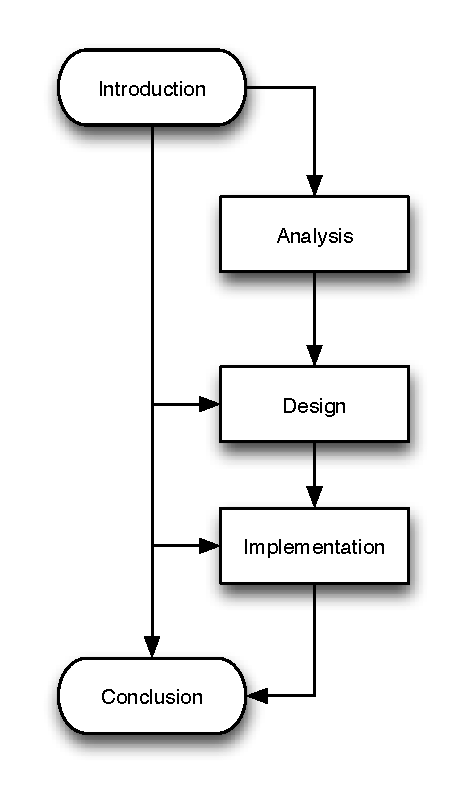
\includegraphics[width=0.5\textwidth]{figures/intro/reading.eps}
			\caption{Reading the thesis.}
			\label{fig:reading:the:thesis}
		\end{figure}



